\documentclass[12pt]{beamer}
\usepackage{algorithmic}
\usepackage[brazil]{babel}
\usepackage[utf8]{inputenc}
\usepackage{graphicx}
\title{FlowShop Scheduling}
\author[Fidêncio,Oshiro,Miranda,Iha]{Fabiano Fidêncio\\ Filipe Oshiro\\ Ricardo Miranda\\ Vitor Massaru Iha}
\institute[IC-UNICAMP]{Instituto de Computação - UNICAMP}
\mode<beamer>{
	\usetheme{CambridgeUS}
}

\begin{document}
\begin{frame}<handout:0>
	\titlepage 
\end{frame}

\AtBeginSection[]
{
\begin{frame}
	\frametitle{Sumário}
	\tableofcontents[currentsection]
\end{frame}
}

\section{O Problema}
\begin{frame}
	\frametitle{O Problema}
	\begin{block}{O que ele é}
		\begin{itemize}
			\item Problema de otimização combinatória.	\pause
			\item Fluxo unidirecional de produtos através de unidades de produção. 	\pause
			\item Não há preempção.	\pause
			\item Produto pode pular um estágio de produção mas sempre mantendo o mesmo sentido de fluxo. \pause
			\item Sequencias de Permutação.	\pause
			\item Objetivo: obter a melhor sequencia de operações minimizando o tempo total de produção. \pause

		\end{itemize}
	\end{block}
\end{frame}
\begin{frame}
	\frametitle{Exemplos}
	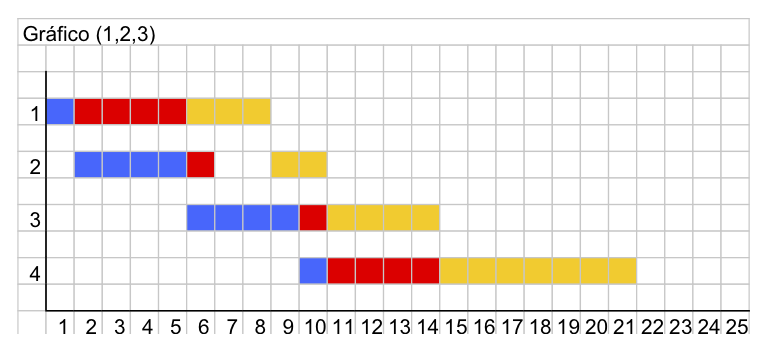
\includegraphics[scale=.6]{graph1} 
\end{frame}
\begin{frame}
	\frametitle{Exemplos}
	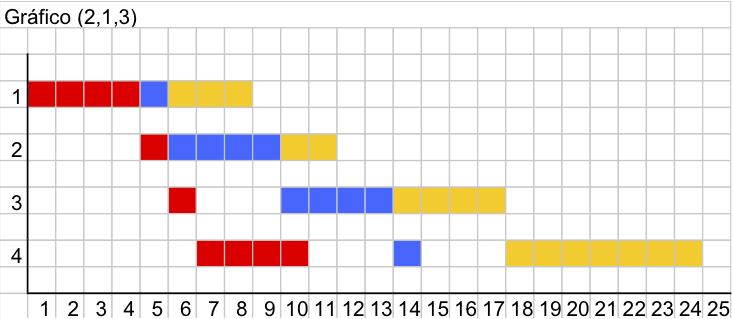
\includegraphics[scale=.6]{graph2} 
\end{frame}
\begin{frame}
	\frametitle{Exemplos}
	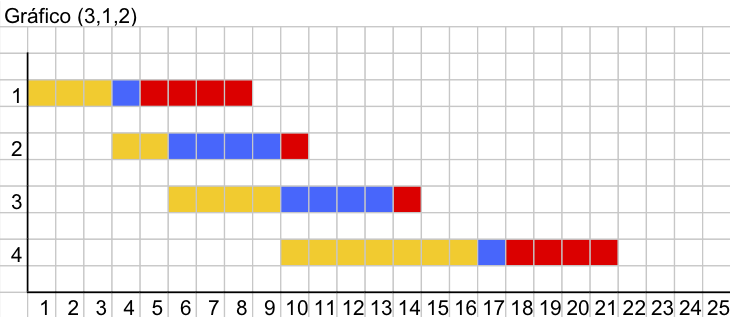
\includegraphics[scale=.6]{graph3} 
\end{frame}
\begin{frame}
	\frametitle{Exemplos}
	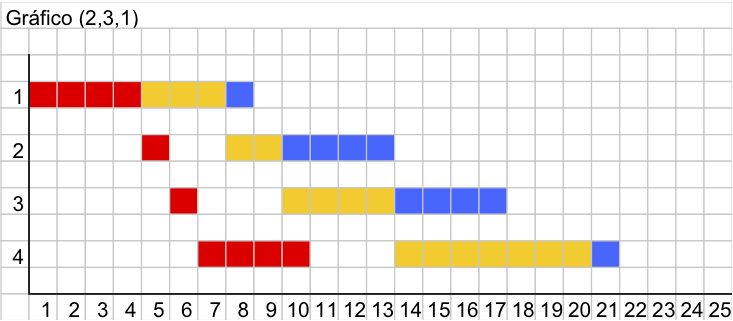
\includegraphics[scale=.6]{graph4} 
\end{frame}
\begin{frame}
	\frametitle{Exemplos}
	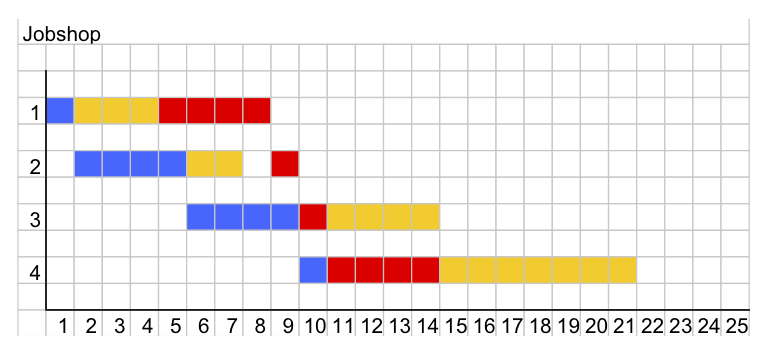
\includegraphics[scale=.6]{graph5} 
\end{frame}
\section{É um problema de IA}
\begin{frame}
        \frametitle{É um problema de IA}
        \begin{block}{}
                \begin{itemize}
                        \item Encontrar a sequência que minimiza o makespan, é um problema NP-difícil   \pause
                        \item Isto inviabiliza a procura pela solução ótima através de algoritmos exatos   \pause
                        \item Abre caminho para a abordagem do problema através de métodos aproximados que procuram encontrar soluções aceitáveis, eventualmente ótimas, em um tempo razoável  \pause
                \end{itemize}
        \end{block}
\end{frame}

\section{Como resolver} 
\begin{frame} 
        \frametitle{Como resolver}
        \begin{block}{Utilizaremos Algoritmos Genéticos para resolução do problema, seguindo o seguite algoritmo base:}
	\end{block}
\end{frame}

\section{Outras abordagens} 
\begin{frame} 
        \frametitle{Outras abordagens}
        \begin{block}{Há algumas outras formas de resolvermos o problema citado, entre elas:}
                \begin{itemize}
                        \item Algoritmo A* (Branch and Bound)    \pause
                        \item Simulated Annealing   \pause
                        \item Busca Tabu  \pause
                \end{itemize}
        \end{block}
\end{frame}
              
\end{document}

